% !TEX root = ../Thesis.tex

\chapter{Additional results}

\section{Small Experiment}

\subsection{GAT-Denoiser components}


\begin{table}[H]
    \centering
    \begin{tabular}{l|c|c|c|c}
      \toprule
      \textbf{Algorithm} & \snrh{ 0} & \snrh{ -5} & \snrh{ -10} & \snrh{ -15} \\
                         & \textbf{SNR} & \textbf{SNR} & \textbf{SNR}  & \textbf{SNR} \\ 
      \midrule
      FBP                 & 4.50 & -0.31  & -5.25 & -10.22  \\ \hline
      BM3D sino           & 9.93 &  7.42  & 4.61  & 2.00    \\ \hline
      BM3D reco           & 10.79 & 8.09  & 4.97  & 1.54    \\ \hline
      U-Net               & 7.13  &  6.18 & 4.34  & 1.87    \\ \hline
      \midrule
      \multicolumn{5}{c}{K-NN k = 8} \\
      GAT                  & 8.32           & 6.94           & 6.19 & 5.01 \\ \hline
      Conv + GAT           & 9.05           & 8.07           & 6.99  & 5.75 \\ \hline
      GAT + U-Net          & 7.49           & 6.40           & 6.01   & 5.07 \\ \hline
      GAT + U-Net**        & 11.88          & \textbf{10.85} & \textbf{9.68} & \textbf{8.26} \\ \hline
      Conv + GAT + U-Net   & 7.55           & 6.50           &5.74 &4.87 \\ \hline
      Conv + GAT + U-Net** & \textbf{11.94} & 10.31          &7.34   &7.33 \\
      \midrule
      \multicolumn{5}{c}{K-NN k = 2} \\
      GAT             &	9.42 	&8.25	&6.78	&5.75  \\
      Conv+GAT        & 10.01 &8.88	&7.69	&6.79  \\
      GAT+U-Net       &	7.93	&7.28	&6.77	&4.91  \\
      GAT+U-Net*      &	11.92	&10.14	&10.13	&8.43 \\
      GAT+U-Net**     &	13.41	&12.12	&10.62	&8.50  \\
      Conv+GAT+U-Net  &	8.17	&7.09	&4.53	&5.67  \\
      Conv+GAT+U-Net* &	12.60	&10.71	&8.80	&8.44  \\
      Conv+GAT+U-Net**&	12.80	&11.70	&10.63	&9.21 \\
    \end{tabular}
  
    \caption{Small Experiment: overall GAT-Denoiser components vs. Baseline for k-NN = 8}
    \label{tab:small_gat_components}
  \end{table}


\subsection{Small experiment - knn with 2 layers, 4 heads}

2 layers, 4 heads

\begin{table}[H]
  \centering
  \begin{tabular}{l|cc}
    \toprule
    \textbf{K-NN parameter k} & \multicolumn{2}{l|}{\snrh{ 0}}   \\
                       & \textbf{Loss} & \textbf{SNR}  \\ 
    \midrule
    2    & 9.90 & 601.38  \\ \hline
    4    & 9.64 & 622.13  \\ \hline
    6    & 9.38 & 634.44  \\ \hline
    8    & 9.19 & 648.97  \\ \hline
    \midrule
  \end{tabular}

  \caption{Different k-NN values for \snry 0 dB and -10 dB }
  \label{tab:small_knn_2}
\end{table}


\subsection{Small experiment - GAT dropout}
\begin{table}[H]
  \centering
  \begin{tabular}{l|cc}
    \toprule
    \textbf{K-NN parameter k} & \multicolumn{2}{l|}{\snrh{ 0}}   \\
                       & \textbf{Loss} & \textbf{SNR}  \\ 
    \midrule
    0       & 8.33 & 739.5  \\ \hline
    0.01    & 7.81 & 766.2  \\ \hline
    0.03    & 7.98 & 743.3  \\ \hline
    0.05    & 8.09 & 738.4  \\ \hline
    0.1     & 7.79 & 761.8  \\ 
    \midrule
  \end{tabular}

  \caption{Different k-NN values for \snry 0 dB and -10 dB }
  \label{tab:small_droput}
\end{table}

\section{Large Scale experiment}

\subsection{Baseline results}

\begin{table}[H]
  \centering
  \begin{tabular}{l|cc|cc|cc|cc}
    \toprule
    \textbf{Algorithm} & \multicolumn{2}{l|}{\snrh{ 0}} & \multicolumn{2}{l|}{\snrh{ -5}} & \multicolumn{2}{l|}{\snrh{ -10}} & \multicolumn{2}{l}{\snrh{ -15}} \\
                       & \textbf{Loss} & \textbf{SNR} & \textbf{Loss} & \textbf{SNR} & \textbf{Loss} & \textbf{SNR} & \textbf{Loss} & \textbf{SNR} \\ 
    \midrule
    FBP                 & 4.57  & 1167.6 & -0.19 & 1973.5 & -5.17 & 3425.3 & -10.09 & 10'737.3       \\ \hline
    BM3D sino           & 9.93  & 709.9  &  7.40 & 890.6  & 4.61  & 1168.0 & 2.09   & 1570.0 \\ \hline
    BM3D reco           & 10.85 & 658.2  & 8.15  & 818.6  & 5.07  & 1118.3 & 1.76   & 1662.5 \\ \hline
    U-Net               & 7.18  &  968.8 & 6.34  & 1044.7 & 4.50  & 1214.1 & 1.94   & 1522.4        \\ 
    \midrule
  \end{tabular}
  \caption{Baseline results large experiments}
  \label{tab:baseline-large}
\end{table}

\subsection{Large scale component results}

\begin{table}[H]
    \centering
    \begin{tabular}{l|c|c|c|c}
      \toprule
      \textbf{Algorithm} & \snrh{ 0} & \snrh{ -5} & \snrh{ -10} & \snrh{ -15} \\
                         & \textbf{SNR} & \textbf{SNR} & \textbf{SNR}  & \textbf{SNR} \\ 
      \midrule
      FBP                 & 4.57   & -0.19  & -5.17  & -10.09 \\ \hline
      BM3D sino           & 9.93   &  7.40  & 4.61   & \textbf{2.09}   \\ \hline
      BM3D reco           & \textbf{10.85}  & \textbf{8.15}   & \textbf{5.07}   & 1.76   \\ \hline
      U-Net               & 7.18   & 6.34   & 4.50   & 1.94   \\ 
      \midrule
      \multicolumn{5}{c}{K-NN k = 2} \\
    
        GAT              & 9.36	& 7.89	& 6.64	& 5.32    \\ \hline
        Conv+GAT         &	10.05	& 9.07	& 7.17	& 6.15    \\ \hline
        GAT+U-Net        &	8.39 	& 7.49	& 6.60	& 5.66    \\ \hline
        GAT+U-Net**      &	13.34	& 12.07	& \textbf{11.46}	& \textbf{9.62}   \\ \hline
        Conv+GAT+U-Net   &	8.31	& 7.47	&6.66	  & 5.15   \\ \hline
        Conv+GAT+U-Net** &	\textbf{13.43}	& \textbf{12.52}	& 11.43	& 9.55   \\ 
    \end{tabular}
  
    \caption{Large scale experiment: overall GAT-Denoiser components vs. Baseline for k-NN = 2}
    \label{tab:large_gat_components_knn2}
  \end{table}

\section{wandb logging:}
\subsection{Small experiment:}
\begin{itemize}
  \item FBP: \url{https://wandb.ai/cedric-mendelin/FBP-Validation-LoDoPaB-small}
  \item BM3D: \url{https://wandb.ai/cedric-mendelin/BM3D-Validation-LoDoPaB-small}
  \item U-Net: \url{https://wandb.ai/cedric-mendelin/U-Net-Validation-LoDoPaB-small}
  \item k-nn and graph structure \url{https://wandb.ai/cedric-mendelin/LoDoPaB-Small-k-NN-and-graph-size}
  \item Conv: \url{https://wandb.ai/cedric-mendelin/LoDoPaB-Small-Convolution}
  \item Loss: \url{https://wandb.ai/cedric-mendelin/LoDoPaB-Small-Loss-FBP-vs-SINO}
  \item Dropout: \url{https://wandb.ai/cedric-mendelin/LoDoPaB-Small-GAT-dropout}
  \item Components k-nn 2: \url{https://wandb.ai/cedric-mendelin/LoDoPaB-Small-Components-knn-2}
  \item Components k-nn 8: \url{https://wandb.ai/cedric-mendelin/LoDoPaB-Small-Components-knn-8}
\end{itemize}

\subsection{Large scale experiments}
\begin{itemize}
  \item U-NET: \url{https://wandb.ai/cedric-mendelin/U-Net-Validation-LoDoPaB-large}
  \item FBP: \url{https://wandb.ai/cedric-mendelin/FBP-Validation-LoDoPaB-large}
  \item BM3D: \url{https://wandb.ai/cedric-mendelin/BM3D-Validation-LoDoPaB-large}
  \item Gat-Denoiser: \url{https://wandb.ai/cedric-mendelin/LoDoPaB-Large-knn-2}
\end{itemize}


\section{Visual Results}

\subsection{Clean images}
\begin{figure}[H]
  \centering
  \hfill
  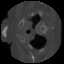
\includegraphics[width=0.16\textwidth]{clean/clean_1.png}
  \hfill
  
\includegraphics[width=0.16\textwidth]{clean/clean_2.png}
  \hfill
  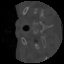
\includegraphics[width=0.16\textwidth]{clean/clean_3.png}
  \hfill
  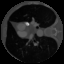
\includegraphics[width=0.16\textwidth]{clean/clean_6.png}
  \hfill
  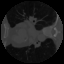
\includegraphics[width=0.16\textwidth]{clean/clean_9.png}
  \hfill
  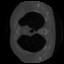
\includegraphics[width=0.16\textwidth]{clean/clean_10.png}
  \hfill
  \caption{FBP reconstruction for \snry 0 dB}
\end{figure}


\subsection{\snry 0 dB}
\visualresults{0}

\subsection{\snry -5 dB}
\visualresults{-5}


\subsection{\snry -10 dB}
\visualresults{-10}


\subsection{\snry -15 dB}
\visualresults{-15}